\begin{center}

\includegraphics[width=0.4\textwidth]{content/3/chapter6/images/28.png}\\
Cippi在唱诗班唱歌
\end{center}

\begin{tcolorbox}[breakable,enhanced jigsaw,colback=blue!5!white,colframe=blue!75!black,title={编译器对同步输出流的支持}]
	
到2020年底,只有GCC 11支持同步输出流。
	
\end{tcolorbox}

若不同步地写入std::cout会发生什么?

\begin{lstlisting}[style=styleCXX]
// coutUnsynchronized.cpp

#include <chrono>
#include <iostream>
#include <thread>

class Worker{
public:
	Worker(std::string n):name(n) {};
	void operator() (){
		for (int i = 1; i <= 3; ++i) {
			// begin work
			std::this_thread::sleep_for(std::chrono::milliseconds(200));
			// end work
			std::cout << name << ": " << "Work " << i << " done !!!" << '\n';
		}
	}
private:
	std::string name;
};


int main() {

	std::cout << '\n';
	
	std::cout << "Boss: Let's start working.\n\n";
	
	std::thread herb= std::thread(Worker("Herb"));
	std::thread andrei= std::thread(Worker(" Andrei"));
	std::thread scott= std::thread(Worker(" Scott"));
	std::thread bjarne= std::thread(Worker(" Bjarne"));
	std::thread bart= std::thread(Worker(" Bart"));
	std::thread jenne= std::thread(Worker(" Jenne"));
	
	
	herb.join();
	andrei.join();
	scott.join();
	bjarne.join();
	bart.join();
	jenne.join();
	
	std::cout << "\n" << "Boss: Let's go home." << '\n';
	
	std::cout << '\n';

}
\end{lstlisting}

老板有六个工人(第29-34行)。每个工作人员必须处理三个工作包,每个工作包花费1/5秒(第13行)。工人完成了他的工作包后,他大声地向老板报告(第15行)。当老板收到所有员工的通知,老板就会把工人们送回家(第44行)。

这么简单的工作流程真是一团糟!每个员工都大声喊出自己的信息,无视其他同事!

\begin{center}
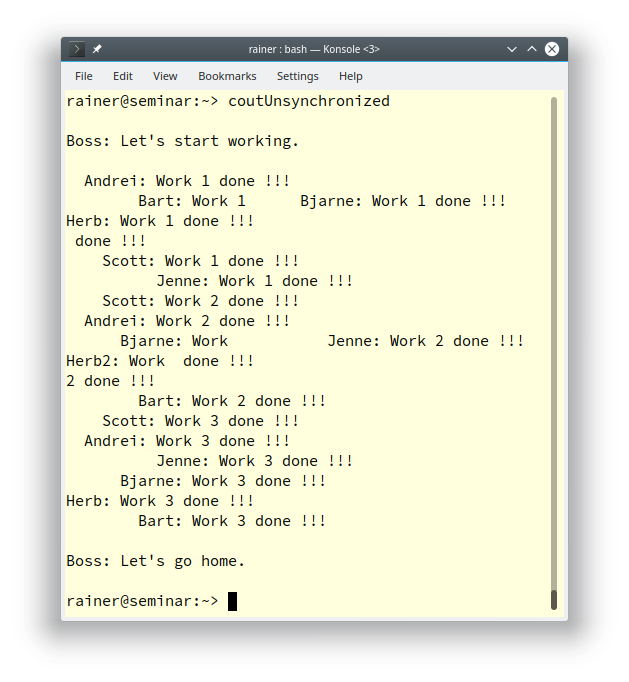
\includegraphics[width=0.6\textwidth]{content/3/chapter6/images/29.png}\\
\end{center}

\begin{tcolorbox}[breakable,enhanced jigsaw,colback=blue!5!white,colframe=blue!75!black,title={std::cout是线程安全的}]
	
C++11标准确定不需要对std::cout进行额外的保护,每个字符都是原子地“输出”。类似于示例中的输出语句可能交织在一起的情况,只是一个视觉问题;而程序定义良好,没有问题。此注释对所有全局流对象有效。插入和提取全局流对象(std::cout, std::cin, std::cerr和std::clog)是线程安全的。更准确地说:写入std::cout并没有参与数据竞争,而是创建了条件竞争,所以由于线程的交错,从而导致了屏幕输出的错乱。
	
\end{tcolorbox}

如何解决这个问题?C++11中,答案很简单:可以使用\href{https://en.cppreference.com/w/cpp/thread/lock_guard}{lock\_guard}这样的锁来同步对std::cout的访问。

\begin{lstlisting}[style=styleCXX]
// coutSynchronized.cpp

#include <chrono>
#include <iostream>
#include <mutex>
#include <thread>

std::mutex coutMutex;

class Worker{
public:
	Worker(std::string n):name(n) {};
	
	void operator() () {
		for (int i = 1; i <= 3; ++i) {
			// begin work
			std::this_thread::sleep_for(std::chrono::milliseconds(200));
			// end work
			std::lock_guard<std::mutex> coutLock(coutMutex);
			std::cout << name << ": " << "Work " << i << " done !!!\n";
		}
	}
private:
	std::string name;
};


int main() {

	std::cout << '\n';
	
	std::cout << "Boss: Let's start working." << "\n\n";
	
	std::thread herb= std::thread(Worker("Herb"));
	std::thread andrei= std::thread(Worker(" Andrei"));
	std::thread scott= std::thread(Worker(" Scott"));
	std::thread bjarne= std::thread(Worker(" Bjarne"));
	std::thread bart= std::thread(Worker(" Bart"));
	std::thread jenne= std::thread(Worker(" Jenne"));
	
	herb.join();
	andrei.join();
	scott.join();
	bjarne.join();
	bart.join();
	jenne.join();
	
	std::cout << "\n" << "Boss: Let's go home." << '\n';
	
	std::cout << '\n';

}
\end{lstlisting}

第8行中的coutMutex保护共享对象std::cout。将coutMutex放入std::lock\_guard中可以保证coutMutex在std::lock\_guard的构造函数(第19行)中被锁定,在std::lock\_guard的析构函数(第21行)中解锁。因为coutLock守护的coutMutex,混乱的输出才会变得和谐。

\begin{center}
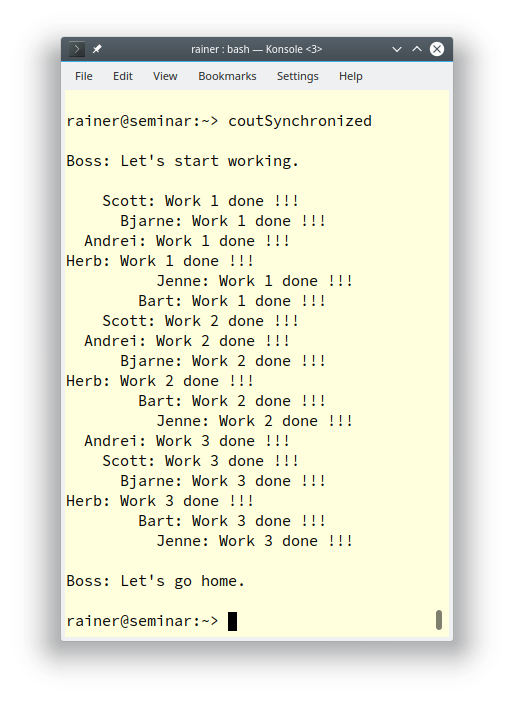
\includegraphics[width=0.6\textwidth]{content/3/chapter6/images/30.png}\\
\end{center}

C++20编写同步的std::cout更是小菜一碟。std::basic\_syncbuf是\href{https://en.cppreference.com/w/cpp/io/basic_streambuf}{std::basic\_streambuf}的包装器,可以在缓冲区中累积输出。包装器在销毁时将其内容设置为包装的缓冲区,所以内容会显示为连续的字符序列,不会发生字符的交错。

通过std::basic\_osyncstream,可以直接同步写入std::cout。

可以创建命名同步输出流。并且,可以对前面的coutUnsynchronized.cpp进行重构,将synchronized写入到std::cout中。

\begin{lstlisting}[style=styleCXX]
// synchronizedOutput.cpp

#include <chrono>
#include <iostream>
#include <syncstream>
#include <thread>

class Worker{
public:
	Worker(std::string n): name(n) {};
	void operator() (){
		for (int i = 1; i <= 3; ++i) {
			// begin work
			std::this_thread::sleep_for(std::chrono::milliseconds(200));
			// end work
			std::osyncstream syncStream(std::cout);
			syncStream << name << ": " << "Work " << i << " done !!!" << '\n';
		}
	}
private:
std::string name;
};


int main() {

	std::cout << '\n';
	
	std::cout << "Boss: Let's start working.\n\n";
	
	std::thread herb= std::thread(Worker("Herb"));
	std::thread andrei= std::thread(Worker(" Andrei"));
	std::thread scott= std::thread(Worker(" Scott"));
	std::thread bjarne= std::thread(Worker(" Bjarne"));
	std::thread bart= std::thread(Worker(" Bart"));
	std::thread jenne= std::thread(Worker(" Jenne"));
	
	
	herb.join();
	andrei.join();
	scott.join();
	bjarne.join();
	bart.join();
	jenne.join();
	
	std::cout << "\n" << "Boss: Let's go home." << '\n';
	
	std::cout << '\n';

}
\end{lstlisting}

对coutUnsynchronized.cpp的唯一更改,是将std::cout包装在std::osyncstream中(第16行)。当std::osyncstream在第18行中超出范围时,将传输字符并刷新std::cout。值得一提的是,主程序中的std::cout调用不会引入数据竞争,因此不需要同步。

因为只在第17行声明了一次syncStream,所以使用临时对象可能更合适。下面的代码片段展示了修改后的调用运算符。

\begin{lstlisting}[style=styleCXX]
void operator()() {
	for (int i = 1; i <= 3; ++i) {
		// begin work
		std::this_thread::sleep_for(std::chrono::milliseconds(200));
		// end work
		std::osyncstream(std::cout) << name << ": " << "Work " << i << " done !!!"
		                            << '\n';
	}
}
\end{lstlisting}

std::basic\_osyncstream syncStream提供了两个有趣的成员函数。

\begin{enumerate}
\item 
syncStream.emit()发出所有缓冲输出并对所有挂起进行刷新。

\item 
syncStream.get\_wrapped()返回一个指向包装缓冲区的指针。
\end{enumerate}

\href{https://en.cppreference.com/w/cpp/io/basic_osyncstream/get_wrapped}{cppreference.com}展示了如何使用get\_wrapped成员函数对不同输出流的输出进行排序。

\begin{lstlisting}[style=styleCXX]
// sequenceOutput.cpp

#include <syncstream>
#include <iostream>

int main() {
	
	std::osyncstream bout1(std::cout);
	bout1 << "Hello, ";
	{
		std::osyncstream(bout1.get_wrapped()) << "Goodbye, " << "Planet!" << '\n';
	} // emits the contents of the temporary buffer

	bout1 << "World!" << '\n';
	
} // emits the contents of bout1
\end{lstlisting}

\begin{tcblisting}{commandshell={}}
Goodbye, Planet!
Hello, World!
\end{tcblisting}

\begin{tcolorbox}[breakable,enhanced jigsaw,colback=mygreen!5!white,colframe=mygreen!75!black,title={总结}]
	
\begin{itemize}
\item 
std::cout是线程安全的,但是当线程并发地写入std::cout时,可能会出现输出操作的交叉。这只是一个视觉问题,而不是数据竞争。

\item 
C++20支持同步输出流,其在内部缓冲区中积累输出,并在原子步骤中写入内容,所以不会发生输出操作交错的情况。
\end{itemize}
	
\end{tcolorbox}



